\section{Pessimistic Concurrency Control} \label{sec:pessimistic}

To provide a baseline against which to compare the performance of HTM, we will
be implementing two different forms of traditional, software-based pessimistic
concurrency control protocols: a lock manager and spin locks.

\subsection{Lock Manager}

Traditional locking schemes make use of a lock manager, which arbitrates access
to records in the key-value store by granting locks to requesting transactions
on a per-entry basis (i.e., each key-value pair has its own lock). A lock
manager consists of a lock table hashed on keys. Each lock record contains a
mode (either read, write, or free) and a list of transactions waiting to acquire
the lock. A transaction may only access a given key-value pair once it has
requested and been granted the appropriate lock, which prevents conflicting
concurrent operations.

When a process requests a lock, the lock manager grants the request if it is
compatible with the lock's mode, where writes are incompatible with reads and
other writes.  When the transaction currently holding the lock releases it, the
lock manager grants the lock to the transaction at the head of the waiting
queue for that lock.

We will prevent deadlocks by enforcing an ordering in which a transaction may
request locks, ensuring that no circular dependencies between transactions
waiting on locks may occur. This works well under our assumption that the read
and write sets of transactions are static, but is difficult if the read and
write sets are dynamic -- a topic which we hope to explore in our project.\\

\subsection{Spin Locks}

In a spin lock scheme, each key-value pair has an associated memory word
representing its lock. Locks are acquired via an atomic test-and-set
primitive. If a transaction attempts test-and-set but it fails because the lock
is already held, the transaction \textit{spins}, or repeatedly attempts to grab
the lock until it succeeds. As for the lock manager, we will implement deadlock
prevention by enforcing an order in which locks must be obtained.

By avoiding the extra work of going through the manager, spin locks can
potentially be faster. However, the obvious disadvantage of spin locks is that
they require ``busy waiting'': when a transaction spins while waiting for a
lock, it is using CPU time without really doing any useful work. This is
primarily a problem in systems with high contention, where it is likely that
multiple transactions will want to access the same key-value pair at the same
time. Prior work \citep{tran2010} has demonstrated using an HTM simulator that
TM peforms well under low contection workloads and spinlocks work well under
high contention workloads. We plan to evaluate how valid this observation is in
a real-world HTM implementation.
%Time required to access a given number of objects using different concurrency
%control protocols, based on their simulation, is shown in \Cref{fig:overhead}. 

% jarulraj: Removed figure for now -- not sure if we can use it
%\begin{figure}[h!] \centering
%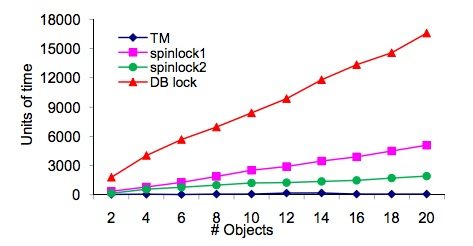
\includegraphics[width=0.45\textwidth]{figure/overhead.jpg} \caption{Overhead
%of different concurrency control protocols under low contention workloads
%\citep{tran2010}.} \label{fig:overhead} \end{figure}
